\documentclass[table]{article}
\usepackage[rgb,dvipsnames]{xcolor}
\usepackage{tikz}
\usepackage{iclr2017_conference,times}
\usepackage{amsmath, amsthm}
\usepackage[subscriptcorrection,mtpcal,amsbb]{mtpro2}
\usepackage{hyperref}
\usepackage{url}
\usepackage{enumitem}
\setlist{leftmargin=15pt}
\usepackage{inconsolata}
\usepackage{textcomp}
\usepackage{lastpage}
\cfoot{\thepage\ of \pageref{LastPage}}
\usepackage{makecell}
\usepackage{physics}
\usetikzlibrary{arrows,positioning,automata}
\usetikzlibrary{shapes.geometric}
\usepackage{float}
\usepackage{subcaption}
\usepackage{array}
\newcolumntype{L}[1]{>{\raggedright\let\newline\\\arraybackslash\hspace{0pt}}m{#1}}
\newcolumntype{C}[1]{>{\centering\let\newline\\\arraybackslash\hspace{0pt}}m{#1}}
\newcolumntype{R}[1]{>{\raggedleft\let\newline\\\arraybackslash\hspace{0pt}}m{#1}}
\usepackage{colortbl}
\usepackage{hhline}
\usepackage[labelfont=bf,labelsep=period]{caption}
\usetikzlibrary{matrix}

\newcommand{\thickhline}{%
    \noalign {\ifnum 0=`}\fi \hrule height 1pt
    \futurelet \reserved@a \@xhline
}

\def\IsEven#1{%
      TT\fi
     \pgfmathparse{int(mod(#1,2))}%
     \ifnum\pgfmathresult=0
}

\lhead{\textsc{IFT6135 Representation Learning}}
\rhead{S. Laferri\`ere \& J. Litalien}

\title{Assignment 4 --- Practical Part \\
Generative Models (GANs)}
\author{Samuel Laferri\`ere\thanks{Student ID P0988904}\ \, \& Joey Litalien\thanks{Student ID P1195712} \\
IFT6135 Representation Learning, Winter 2018\\
Universit\'e de Montr\'eal\\
Prof. Aaron Courville \\
\texttt{$\{$samuel.laferriere.cyr,joey.litalien$\}$@umontreal.ca}}

\def\*#1{\mathbf{#1}}
\DeclareMathOperator{\ex}{\mathbb{E}}
\DeclareMathOperator{\Var}{Var}
\DeclareMathOperator{\KL}{\textit{D}_\mathsf{KL}}
\DeclareMathOperator{\IS}{\mathsf{IS}}
\DeclareMathOperator{\MS}{\mathsf{MS}}

\newcommand{\code}[1]{{\color{Blue}\small\texttt{#1}}}

\begin{document}
\maketitle
\thispagestyle{empty}

\section{Overview}

For this assignment, we chose to implement in PyTorch a Generative Adversarial Network (GAN) as first introduced by \cite{gan}. The variant we used for comparison is a Wasserstein GAN (WGAN) from \cite{wgan}. The class \code{DCGAN} implements a Deep Convolutional GAN and contains both a \code{Discriminator} $D$ and \code{Generator} $G$. Both entities can be trained independently using the methods \code{DCGAN.train\_*}, meaning that we can customize the number of times we update each model. These training routines implement three types of loss functions: the original minmax loss, the Wasserstein loss and the least squares lost from \cite{lsgan}. The last GAN type will not be evaluated in this assignment, but generated images from our LSGAN are available in the Appendix.

Every hyperparameter related to training (\textit{e.g.} learning rate and momentum) is set in \code{CelebA}, a wrapper class for the generative task at hand. To load a pre-trained generative model and sample images from its distribution, simply instantiate \code{DCGAN}, call \code{DCGAN.load_model(fname)} with the saved PyTorch weights, and run \code{DCGAN.generate_img(n)}.

%If no arguments is passed, the GAN will sample a random latent variable $\*z$ and return a generated image. This function also accepts a latent variable generated from a fixed RNG seed.

\section{Architecture}
\subsection{Training the Networks}

We took inspiration from the DCGAN architecture from \cite{dcgan} to build our two GANs. The architectures for the discriminator and generator are given in the tables below and are used on both our vanilla DCGAN and our WGAN. The middle columns are kernel size $(k)$, stride $(s)$ and zero-padding $(p)$, respectively.

\begin{table}[ht]
\centering
\begin{tabular}{c c ccc c c c}
\Xhline{2\arrayrulewidth}
In & Out & Module & $k$ & $s$ & $p$ & Normalization & Activation \\
\hline
100 & 512 &Linear + Reshape &&&& BatchNorm1D & ReLU \\
512 & 256 &ConvTranspose2D & 4 & 2 & 1 & BatchNorm2D & ReLU  \\
128 & 64 &ConvTranspose2D & 4 & 2 & 1 & BatchNorm2D & ReLU  \\
64 & 3 &ConvTranspose2D & 4 & 2 & 1 & None & Tanh\\
\Xhline{2\arrayrulewidth}
\end{tabular}
\caption{DCGAN Generator architecture.}
\end{table}

\begin{table}[ht]
\centering
\begin{tabular}{c c ccc c c c}
\Xhline{2\arrayrulewidth}
In & Out & Module & $k$ & $s$ & $p$ & Normalization & Activation  \\
\hline
3 & 64 &Conv2D & 4 & 2 & 1 & None & LeakyReLU \\
64 & 128 &Conv2D & 4 & 2 & 1 & BatchNorm2D & LeakyReLU \\
128 & 256 &Conv2D & 4 & 2 & 1 & BatchNorm2D & LeakyReLU \\
256 & 512 &Conv2D & 4 & 2 & 1 & BatchNorm2D & LeakyReLU \\
512 & 1 & Conv2D & 4 & 1 & 0& None & None \\
\Xhline{2\arrayrulewidth}
\end{tabular}
\caption{DCGAN Discriminator architecture}
\end{table}

As suggested in the paper, we did not apply batchnorm to $G$'s output layer and $D$'s input layer to avoid sample oscillation and model instability. The latent variable is first project to a $512 \times 4 \times 4 = 8192$-dimensional vector using a dense layer and then reshaped to a volume of $512 \times 4 \times 4$ for the first fractionally-strided convolution. We used a kernel size of 4 instead of 5 and removed all biases in the generator network to speed up the computations.

We further detail our choice of hyperparameters as follows.


\begin{table}[ht]
\centering
\begin{tabular}{l C{1.5cm} c c}
\Xhline{2\arrayrulewidth}
Hyperparameter & Symbol & DCGAN & WGAN \\
\hline
Learning rate & $\alpha$ & $2 \times 10^{-4}$ & $5 \times 10^{-5}$ \\
Momentum & $\beta, \beta^2$ & 0.5, 0.999 & None \\
SGD Optimizers & --- & Adam  & RMSProp \\
$D/G$ updates ratio & $n_{\textsf{critic}}$ & 1 & 5 \\
\Xhline{2\arrayrulewidth}
\end{tabular}
\caption{Training hyperparameters for DCGAN and WGAN}
\end{table}

These parameters are the ones suggested by the original authors and tested on the LSUN dataset. We experimented with different values (\textit{e.g.} Adam for WGAN) but GANs being incredibly hard to train, we settled for these values. Theoretically, the discriminator in a WGAN should be fully converged to get the best estimate of the Wasserstein distance but in practice this does not work so well. Hence, if $G_\textsf{iter}$ is the number of times $G$ has been updated so far in the training and $n_\textsf{critic}$ is the number of times $D$ is updated before $G$ is updated once, we started with $n_\textsf{critic} = 20$ for $G_\textsf{iter} < 50$ (1000 minibatches) or whenever $G_\textsf{iter}+1 \pmod{500} = 0$. This number is reduced to 5 otherwise. This is rather arbitrary but somewhat follows the heuristic described by Arjovsky himself on his \href{https://github.com/martinarjovsky/wassersteingan}{GitHub repo} of the original WGAN.

The dataset contains 202\,599 RGB images of size $3 \times 64 \times 64$. These faces were first normalized and fed into our networks in minibatches of size 64. To train these models, we provided Shell scripts that accept a number of arguments for the optimizers, learning rate, CUDA switch, RNG seed (for debugging), and much more. These are located in \code{src/train}. Below are the training times for our models.

\begin{table}[ht]
\centering
\begin{tabular}{l c c c}
\Xhline{2\arrayrulewidth}
Model & Training time & Avg epoch time & Avg batch time \\
\hline
Vanilla GAN & 3 hrs 34 mins & 4 mins 15 s & 56 ms  \\
WGAN & 2 hrs 38 mins & 3 mins 9 s & 35 ms \\
\Xhline{2\arrayrulewidth}
\end{tabular}
\caption{Training our vanilla GAN and Wassterstein GAN on an NVIDIA GTX 1080}
\end{table}

Animations of the 50 epochs with fixed latent variables can be found in \code{src/checkpoints} under each model's \code{video} folder.

\subsection{Increasing the Feature Map Size}

To illustrate the three upsampling schemes, we reuse a toy example from \cite{odena2016deconvolution}. Here, we used a stride of $s=1$ (in white) and a constant kernel $k=(a,b,c) = \big(\frac{1}{3}, \frac{1}{3},\frac{1}{3}\big)$ of size 3 (in blue). The input vector $\*x$ (in pink) is a discretized color gradient, \textit{i.e.} $\*x = (9,7,5,3,1) \odot 10^{-1} \*1_5$. The upsampled vector $\*y$ is obtained from the matrix $\*C^\top$ and $\*{\hat x}$.

Given an input vector, a fractionally-strided convolution first adds a stride inbetween elements, and then performs a convolution (in blue). We represent this in Figure \ref{fsc}, noting that the kernel is flipped. We also represent $\*C^\top$ as a $4 \times 3$ sparse matrix, mapping from $\*x_{1:3}$ to $\*{\hat x_{2:5}}$. Note the \textit{checkerboard effect} present in $\*y$ due to kernel overlapping.


\newpage
\begin{figure}[ht]
  \centering
  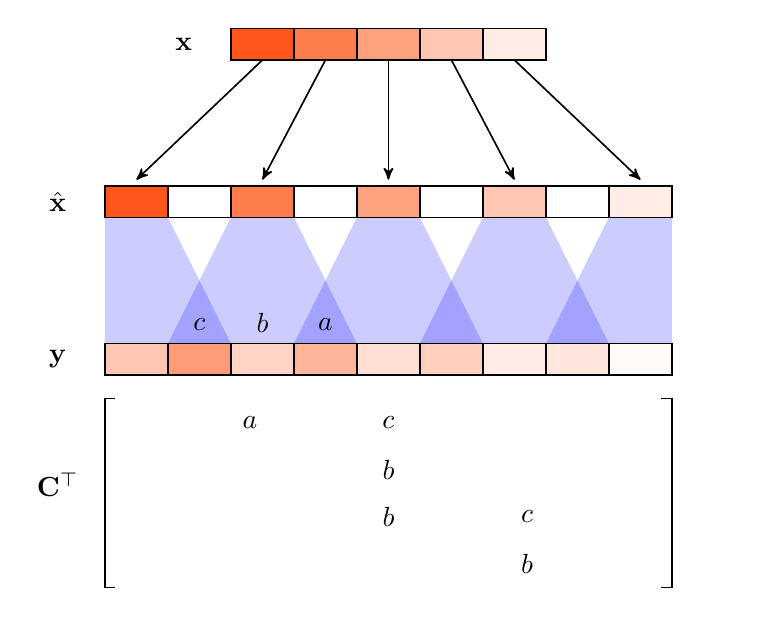
\begin{tikzpicture}[scale=0.8, semithick,  >=stealth']
    \def\x{5}
    \def\y{2.5}
    % Beams
    \foreach \xi in {3,5,7}
      \fill[blue, opacity=0.2] (\xi, \y) -- (\xi+1, 0.5) -- (\xi-2, 0.5) -- (\xi-1, \y);
    % Side beams
    \fill[blue, opacity=0.2] (1, \y) -- (2, 0.5) -- (0, 0.5) -- (0, \y);
    \fill[blue, opacity=0.2] (8, \y) -- (7, 0.5) -- (9, 0.5) -- (9, \y);
    % Pixels
    \foreach \xi[count=\i] in {0,...,8}{
      \if\IsEven{\i}
        \draw[draw=black, fill=gray!75] (\xi,0) rectangle ++(1,0.5);
        \draw[draw=black] (\xi,\y) rectangle ++(1,0.5);
      \else
       % \draw[draw=black, fill=OrangeRed!90] (\xi,\y) rectangle ++(1,0.5);
      \fi
    }
    \draw[draw=black, fill=OrangeRed!30] (0,0) rectangle ++(1,0.5);
    \draw[draw=black, fill=OrangeRed!53] (1,0) rectangle ++(1,0.5);
    \draw[draw=black, fill=OrangeRed!23] (2,0) rectangle ++(1,0.5);
    \draw[draw=black, fill=OrangeRed!40] (3,0) rectangle ++(1,0.5);
    \draw[draw=black, fill=OrangeRed!17] (4,0) rectangle ++(1,0.5);
    \draw[draw=black, fill=OrangeRed!26] (5,0) rectangle ++(1,0.5);
    \draw[draw=black, fill=OrangeRed!10] (6,0) rectangle ++(1,0.5);
    \draw[draw=black, fill=OrangeRed!13] (7,0) rectangle ++(1,0.5);
    \draw[draw=black, fill=OrangeRed!3] (8,0) rectangle ++(1,0.5);

    % Original vector
    \draw[draw=black, fill=OrangeRed!90] (2,2*\y) rectangle ++(1,0.5);
    \draw[draw=black, fill=OrangeRed!70] (3,2*\y) rectangle ++(1,0.5);
    \draw[draw=black, fill=OrangeRed!50] (4,2*\y) rectangle ++(1,0.5);
    \draw[draw=black, fill=OrangeRed!30] (5,2*\y) rectangle ++(1,0.5);
    \draw[draw=black, fill=OrangeRed!10] (6,2*\y) rectangle ++(1,0.5);
    % Middle
    \draw[draw=black, fill=OrangeRed!90] (0,\y) rectangle ++(1,0.5);
    \draw[draw=black, fill=OrangeRed!70] (2,\y) rectangle ++(1,0.5);
    \draw[draw=black, fill=OrangeRed!50] (4,\y) rectangle ++(1,0.5);
    \draw[draw=black, fill=OrangeRed!30] (6,\y) rectangle ++(1,0.5);
    \draw[draw=black, fill=OrangeRed!10] (8,\y) rectangle ++(1,0.5);

    % Arrows
    \draw[->] (2.5, 2*\y) -- (0.5, \y+0.6);
    \draw[->] (3.5, 2*\y) -- (2.5, \y+0.6);
    \draw[->] (4.5, 2*\y) -- (4.5, \y+0.6);
    \draw[->] (5.5, 2*\y) -- (6.5, \y+0.6);
    \draw[->] (6.5, 2*\y) -- (8.5, \y+0.6);
    % Kernel labels
    \node at (3.5,0.8) {$a$};
    \node at (2.5,0.83) {$b$};
    \node at (1.5,0.8) {$c$};
    % Node labels
    \node at (2-0.75,2*\y+0.25) {$\*x$};
    \node at (-0.75,\y+0.25) {$\hat{\*x}$};
    \node at (-0.75,0.25) {$\*y$};
    \node at (-0.75,-2+0.25) {$\*C^\top$};
    \node[opacity=0] at (10,0) {\phantom{0}};
    % Matrix
    \def\d{-0.75}
    \def\e{0.5}
    \node at (1.8+\e,\d) {$a$};
    \node at (4+\e,\d) {$c$};
    \node at (4+\e,2*\d) {$b$};
    \node at (4+\e,3*\d) {$b$};
    \node at (6.2+\e,3*\d) {$c$};
    \node at (6.2+\e,4*\d) {$b$};
    \draw (\e/3,\d/2) -- (0,\d/2) -- (0,4*\d + \d/2) -- (\e/3, 4*\d + \d/2);
    \draw (9-\e/3,\d/2) -- (9,\d/2) -- (9,4*\d + \d/2) -- (9-\e/3, 4*\d + \d/2);
  \end{tikzpicture}
\caption{Fractionally-strided convolution}
\label{fsc}
\end{figure}

In the case of a nearest neighbor (NN) resize convolution, we first expand $\*x$ by duplicating the elements to obtain $\hat{\*x}$ and then perform the convolution. Doing the arithmetic gives us the matrix $\*C^\top$ depicted in Figure \ref{nnc} below. We observe that the upsampled vector $\*y$ is much smoother and is free of any artifact other than at its extremes.

\begin{figure}[ht]
  \centering
  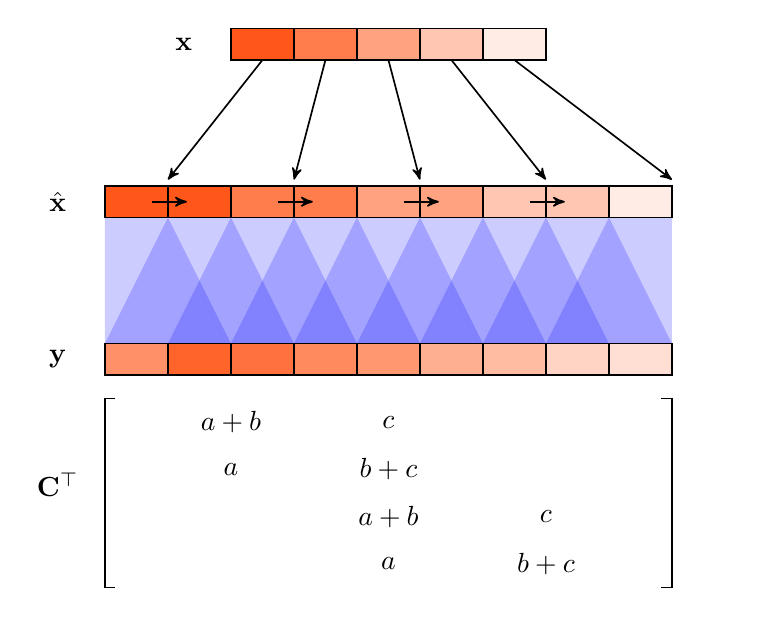
\begin{tikzpicture}[scale=0.8, semithick, >=stealth']
    \def\x{5}
    \def\y{2.5}
    % Beams
    \foreach \xi in {2,...,8}
      \fill[blue, opacity=0.2] (\xi, \y) -- (\xi+1, 0.5) -- (\xi-2, 0.5) -- (\xi-1, \y);
    % Side beams
    \fill[blue, opacity=0.2] (1, \y) -- (2, 0.5) -- (0, 0.5) -- (0, \y);
    \fill[blue, opacity=0.2] (8, \y) -- (7, 0.5) -- (9, 0.5) -- (9, \y);
    % Bottom dark
    \foreach \xi[count=\i] in {1,...,7}{
      \draw[draw=black, fill=gray!75] (\xi,0) rectangle ++(1,0.5);
    }

    \draw[draw=black, fill=OrangeRed!90] (0,\y) rectangle ++(1,0.5);
    \draw[draw=black, fill=OrangeRed!90] (1,\y) rectangle ++(1,0.5);
    \draw[draw=black, fill=OrangeRed!70] (2,\y) rectangle ++(1,0.5);
    \draw[draw=black, fill=OrangeRed!70] (3,\y) rectangle ++(1,0.5);
    \draw[draw=black, fill=OrangeRed!50] (4,\y) rectangle ++(1,0.5);
    \draw[draw=black, fill=OrangeRed!50] (5,\y) rectangle ++(1,0.5);
    \draw[draw=black, fill=OrangeRed!30] (6,\y) rectangle ++(1,0.5);
    \draw[draw=black, fill=OrangeRed!30] (7,\y) rectangle ++(1,0.5);
    \draw[draw=black, fill=OrangeRed!10] (8,\y) rectangle ++(1,0.5);

    \draw[draw=black, fill=OrangeRed!90] (2,2*\y) rectangle ++(1,0.5);
    \draw[draw=black, fill=OrangeRed!70] (3,2*\y) rectangle ++(1,0.5);
    \draw[draw=black, fill=OrangeRed!50] (4,2*\y) rectangle ++(1,0.5);
    \draw[draw=black, fill=OrangeRed!30] (5,2*\y) rectangle ++(1,0.5);
    \draw[draw=black, fill=OrangeRed!10] (6,2*\y) rectangle ++(1,0.5);

    % Bottom
    \draw[draw=black, fill=OrangeRed!59] (0,0) rectangle ++(1,0.5);
    \draw[draw=black, fill=OrangeRed!83] (1,0) rectangle ++(1,0.5);
    \draw[draw=black, fill=OrangeRed!76] (2,0) rectangle ++(1,0.5);
    \draw[draw=black, fill=OrangeRed!63] (3,0) rectangle ++(1,0.5);
    \draw[draw=black, fill=OrangeRed!56] (4,0) rectangle ++(1,0.5);
    \draw[draw=black, fill=OrangeRed!43] (5,0) rectangle ++(1,0.5);
    \draw[draw=black, fill=OrangeRed!36] (6,0) rectangle ++(1,0.5);
    \draw[draw=black, fill=OrangeRed!23] (7,0) rectangle ++(1,0.5);
    \draw[draw=black, fill=OrangeRed!17] (8,0) rectangle ++(1,0.5);

    \draw[->] (2.5, 2*\y) -- (1, \y+0.6);
    \draw[->] (3.5, 2*\y) -- (3, \y+0.6);
    \draw[->] (4.5, 2*\y) -- (5, \y+0.6);
    \draw[->] (5.5, 2*\y) -- (7, \y+0.6);
    \draw[->] (6.5, 2*\y) -- (9, \y+0.6);
    % Arrows
    \foreach \xi[count=\i] in {0,2,4,6}{
      \draw[->] (\xi+0.75, \y+0.25) -- (\xi+1.3, \y+0.25);
    }
     % Node labels
    \node at (2-0.75,2*\y+0.25) {$\*x$};
    \node at (-0.75,\y+0.25) {$\hat{\*x}$};
    \node at (-0.75,0.25) {$\*y$};
    \node at (-0.75,-2+0.25) {$\*C^\top$};
    \node[opacity=0] at (10,0) {\phantom{0}};
    % Matrix
    \def\d{-0.75}
    \def\e{0.5}
    \node at (1.5+\e,\d) {$a+b$};
    \node at (1.5+\e,2*\d) {$a$};
    \node at (4+\e,\d) {$c$};
    \node at (4+\e,2*\d) {$b+c$};
    \node at (4+\e,3*\d) {$a+b$};
    \node at (4+\e,4*\d) {$a$};
    \node at (6.5+\e,3*\d) {$c$};
    \node at (6.5+\e,4*\d) {$b+c$};
    \draw (\e/3,\d/2) -- (0,\d/2) -- (0,4*\d + \d/2) -- (\e/3, 4*\d + \d/2);
    \draw (9-\e/3,\d/2) -- (9,\d/2) -- (9,4*\d + \d/2) -- (9-\e/3, 4*\d + \d/2);
  \end{tikzpicture}
  \caption{Nearest-neighbor upsampling + Convolution}
  \label{nnc}
\end{figure}

Finally, the bilinear resize convolution maps $\*x$ to $\hat{\*x}$ by interpolating between the values. This introduces $\frac{1}{2}$ terms in the deconvolution matrix which needs to be $4 \times 4$ in this case. This is shown in Figure \ref{brc}.

\begin{figure}[ht]
  \centering
  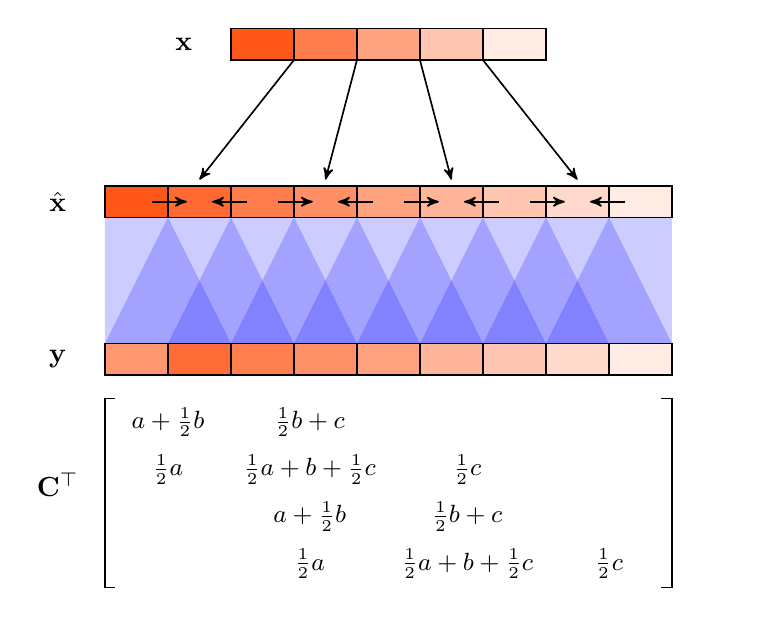
\begin{tikzpicture}[scale=0.8, semithick, >=stealth']
    \def\x{5}
    \def\y{2.5}
    % Beams
    \foreach \xi in {2,...,8}
      \fill[blue, opacity=0.2] (\xi, \y) -- (\xi+1, 0.5) -- (\xi-2, 0.5) -- (\xi-1, \y);
    % Side beams
    \fill[blue, opacity=0.2] (1, \y) -- (2, 0.5) -- (0, 0.5) -- (0, \y);
    \fill[blue, opacity=0.2] (8, \y) -- (7, 0.5) -- (9, 0.5) -- (9, \y);
    % Pixels
    \foreach \xi[count=\i] in {0,...,8}{
      \if\IsEven{\i}
      \else
        \draw[draw=black, fill=gray!25] (\xi,0) rectangle ++(1,0.5);
      \fi
    }

    \draw[draw=black, fill=OrangeRed!90] (0,\y) rectangle ++(1,0.5);
    \draw[draw=black, fill=OrangeRed!80] (1,\y) rectangle ++(1,0.5);
    \draw[draw=black, fill=OrangeRed!70] (2,\y) rectangle ++(1,0.5);
    \draw[draw=black, fill=OrangeRed!60] (3,\y) rectangle ++(1,0.5);
    \draw[draw=black, fill=OrangeRed!50] (4,\y) rectangle ++(1,0.5);
    \draw[draw=black, fill=OrangeRed!40] (5,\y) rectangle ++(1,0.5);
    \draw[draw=black, fill=OrangeRed!30] (6,\y) rectangle ++(1,0.5);
    \draw[draw=black, fill=OrangeRed!20] (7,\y) rectangle ++(1,0.5);
    \draw[draw=black, fill=OrangeRed!10] (8,\y) rectangle ++(1,0.5);

    \draw[draw=black, fill=OrangeRed!90] (2,2*\y) rectangle ++(1,0.5);
    \draw[draw=black, fill=OrangeRed!70] (3,2*\y) rectangle ++(1,0.5);
    \draw[draw=black, fill=OrangeRed!50] (4,2*\y) rectangle ++(1,0.5);
    \draw[draw=black, fill=OrangeRed!30] (5,2*\y) rectangle ++(1,0.5);
    \draw[draw=black, fill=OrangeRed!10] (6,2*\y) rectangle ++(1,0.5);


    % Bottom
    \draw[draw=black, fill=OrangeRed!56] (0,0) rectangle ++(1,0.5);
    \draw[draw=black, fill=OrangeRed!79] (1,0) rectangle ++(1,0.5);
    \draw[draw=black, fill=OrangeRed!69] (2,0) rectangle ++(1,0.5);
    \draw[draw=black, fill=OrangeRed!59] (3,0) rectangle ++(1,0.5);
    \draw[draw=black, fill=OrangeRed!50] (4,0) rectangle ++(1,0.5);
    \draw[draw=black, fill=OrangeRed!40] (5,0) rectangle ++(1,0.5);
    \draw[draw=black, fill=OrangeRed!30] (6,0) rectangle ++(1,0.5);
    \draw[draw=black, fill=OrangeRed!20] (7,0) rectangle ++(1,0.5);
    \draw[draw=black, fill=OrangeRed!10] (8,0) rectangle ++(1,0.5);

    \draw[->] (3, 2*\y) -- (1.5, \y+0.6);
    \draw[->] (4, 2*\y) -- (3.5, \y+0.6);
    \draw[->] (5, 2*\y) -- (5.5, \y+0.6);
    \draw[->] (6, 2*\y) -- (7.5, \y+0.6);
    % Node labels
    \node at (2-0.75,2*\y+0.25) {$\*x$};
    \node at (-0.75,\y+0.25) {$\hat{\*x}$};
    \node at (-0.75,0.25) {$\*y$};
    \node at (-0.75,-2+0.25) {$\*C^\top$};
    \node[opacity=0] at (10,0) {\phantom{0}};
    % Arrows
    \foreach \xi[count=\i] in {0,2,4,6}{
      \draw[->] (\xi+0.75, \y+0.25) -- (\xi+1.3, \y+0.25);
      \draw[->] (\xi+2.25, \y+0.25) -- (\xi+1.7, \y+0.25);
    }
    % Matrix
    \def\d{-0.75}
    \def\e{0.5}
    \node at (0.5+\e,\d) {\small$a+\frac{1}{2}b$};
    \node at (0.5+\e,2*\d) {\small$\frac{1}{2}a$};
    \node at (2.75+\e,\d) {\small$\frac{1}{2}b + c$};
    \node at (2.75+\e,2*\d) {\small$\frac{1}{2}a + b + \frac{1}{2}c$};
    \node at (2.75+\e,3*\d) {\small$a+\frac{1}{2}b$};
    \node at (2.75+\e,4*\d) {\small$\frac{1}{2}a$};
    \node at (5.25+\e,3*\d) {\small$\frac{1}{2}b+c$};
    \node at (5.25+\e,2*\d) {\small$\frac{1}{2}c$};
    \node at (5.25+\e,4*\d) {\small$\frac{1}{2}a + b+\frac{1}{2}c$};
    \node at (7.5+\e,4*\d) {\small$\frac{1}{2}c$};
    \draw (\e/3,\d/2) -- (0,\d/2) -- (0,4*\d + \d/2) -- (\e/3, 4*\d + \d/2);
    \draw (9-\e/3,\d/2) -- (9,\d/2) -- (9,4*\d + \d/2) -- (9-\e/3, 4*\d + \d/2);
  \end{tikzpicture}
  \caption{Bilinear upsampling + Convolution}
  \label{brc}
\end{figure}

\newpage
\section{Qualitative Evaluations}
\subsection{DCGAN vs. WGAN Visual Comparison}
\begin{figure}[ht]
  \centering
  \begin{subfigure}{\textwidth}
    \centering
    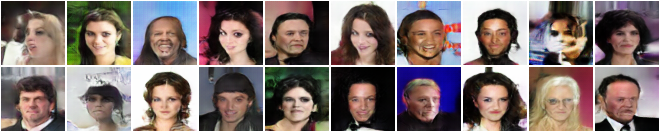
\includegraphics[scale=0.5]{imgs/gan_examples}
    \caption{Vanilla GAN}
  \end{subfigure}

  \vspace*{3mm}
  \begin{subfigure}{\textwidth}
    \centering
    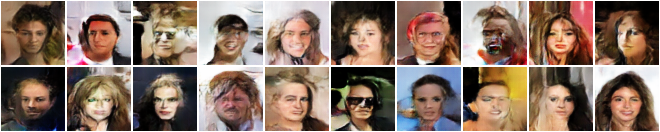
\includegraphics[scale=0.5]{imgs/wgan_examples}
    \caption{WGAN}
  \end{subfigure}
  \caption{Comparing our vanilla GAN (\textit{top}) with its Wasserstein counterpart (\textit{bottom}). More images can be found in the Appendix.}
    \label{compare}
\end{figure}

Against all odds, it seems like our GAN outperforms our WGAN. Even if the latter does not show any sign of partial mode collapse as compared to the former (so more diverse, see Appendix), the quality of the samples produced by the vanilla DCGAN are clearly superior. Our GAN's outputs are more crisp and less blurry. In particular, the Wasserstein GAN samples look more like oil paintings and very few samples could be confused with an actual human face. It is unclear why this is the case, as with anything related to GANs really.

To improve our models, the main direction would be to use bigger images (\textit{e.g.} $3 \times 128 \times 128$) and experiment more with the heuristic used for setting $n_\textsf{critic}$ in the contect of WGANs. In particular, monitoring the loss more closely could ensure our generator converges. Another possibility would be to use gradient penalty from \cite{wgangp} instead of weight clipping to enforce the Lipschitz constraint. One final possibility would be to go deeper and add an extra layer in the discriminator architecture so that the sequence goes $100 \to 1024 \to 512 \to \cdots$ instead of $100 \to 512 \to \cdots$.


\subsection{Latent Space Exploration}
To explore the face manifold in latent space, we iterated over all $10^2$ dimensions of two given $\*z$'s and changed the value to $\pm 3\sigma^2 = \pm 3$ to amplify the signal. We selected the dimensions we thought gave the most notable differences and plotted them in Figure \ref{latent_explore}. Some of the visual variations we observed are open/close mouth, skin color, hair fringe, hair colour, cheek and jaw shape, background, and gender changes. Interestingly, we also have a semblance of face rotation with the woman in the Vanilla GAN (first and fourth from the right).
\begin{figure}[ht]
  \centering
  \begin{subfigure}{\textwidth}
    \centering
    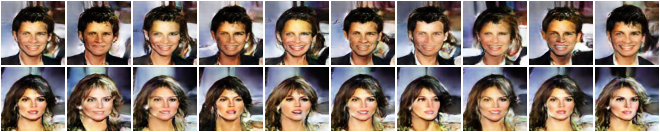
\includegraphics[scale=0.5]{imgs/gan_latent_play}
    \caption{Vanilla GAN}
  \end{subfigure}

  \vspace*{3mm}
  \begin{subfigure}{\textwidth}
    \centering
    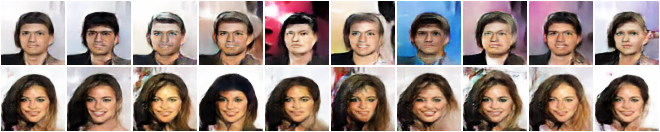
\includegraphics[scale=0.5]{imgs/wgan_latent_play}
    \caption{WGAN}
  \end{subfigure}
  \caption{Changing a single dimension in latent space for different generative models. Original face $\*x = G(\*z)$ is the left-most image.}
  \label{latent_explore}
\end{figure}

Note that we had to handpick the samples for the WGAN given the poor quality of the model. It is still interesting to see that the latent space exploration somewhat gives sensible results even when the model's generative performance is poor. One could try to experiment with higher dimensional changes (\textit{e.g.} moving many dimensions at once) as well.

\subsection{Screen and Latent Space Interpolation}
Interpolating in screen space (Fig. \ref{screen_lerp}) obviously gave very poor results as we simply interpolate between pixels and completely disregard the underlying structure of the generator $G$. Only the first and last images look like actual human faces; anything in the middle has ghosting artifacts since it is just a blend of RGB channels.

% WGAN: Seed 5 35
% 86 112
% 140 186
% 229 278
Interpolating in latent space (Fig. \ref{latent_lerp}), however, gives pleasant results. Indeed, any $\*z'$ seems to yield a plausible celebrity face. This is because when we interpolate the latent variables, we ``walk" on the face manifold of $G$ and so any value should somewhat give a realistic face.

To better visualize the interpolation process, we created looping GIFs (and MP4 videos to avoid compression artifacts) over 50 frames (\textit{i.e.} $\alpha = i/50$). These are located in the \code{explore/screen\_space} and \code{explore/latent\_space} directories of the project source. You can create an interpolating sequence between two random seeds by running the provided Python script with a pretrained generative model. A series of arguments such as model type and number of frames can be specified. For more info, simply run the program with the help flag.

\clearpage
\begin{figure}
  \centering
  \begin{subfigure}{\textwidth}
    \centering
    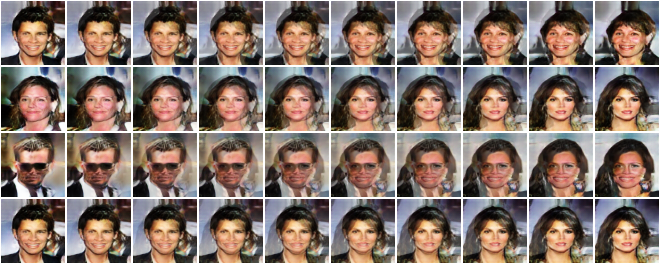
\includegraphics[scale=0.5]{imgs/gan_screen_lerp}
    \caption{Vanilla GAN}
  \end{subfigure}

  \vspace*{3mm}
  \begin{subfigure}{\textwidth}
    \centering
    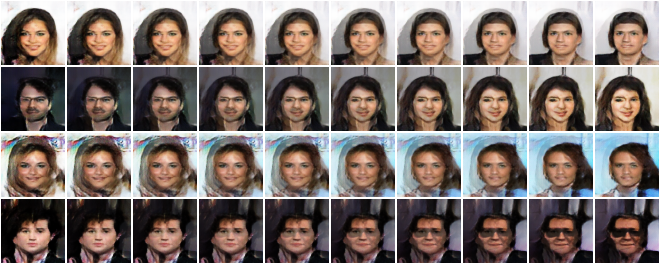
\includegraphics[scale=0.5]{imgs/wgan_screen_lerp}
    \caption{WGAN}
  \end{subfigure}
  \caption{Interpolating in screen space for different generative models. Each image is generated using two fixed latent variables and computing $\*x' = \alpha \*x_0 + (1-\alpha)\*x_1, \ \alpha \in [0,1]$.}
  \label{screen_lerp}
\end{figure}

\newpage
\clearpage
\begin{figure}
  \centering
  \begin{subfigure}{\textwidth}
    \centering
    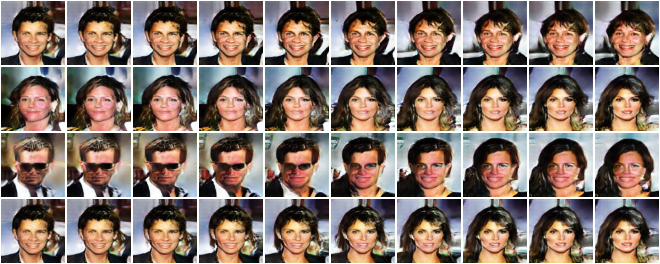
\includegraphics[scale=0.5]{imgs/gan_latent_lerp}
    \caption{Vanilla GAN}
  \end{subfigure}

  \vspace*{3mm}
  \begin{subfigure}{\textwidth}
    \centering
    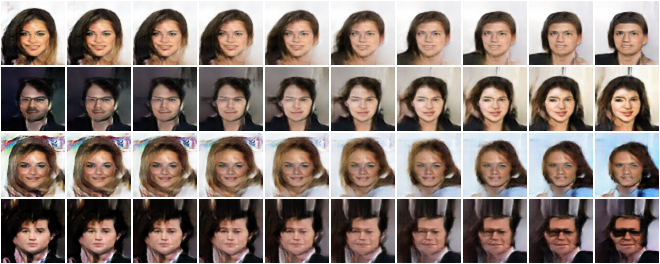
\includegraphics[scale=0.5]{imgs/wgan_latent_lerp}
    \caption{WGAN}
  \end{subfigure}
  \caption{Interpolating in latent space for different generative models. Each image is generated using a different latent variable $\*z' = \alpha \*z_0 + (1-\alpha)\*z_1, \ \alpha \in [0,1]$.}
  \label{latent_lerp}
\end{figure}

\clearpage
\newpage
\section{Quantitative Evaluations}
\subsection{Results for Inception and Mode Score}
We computed the Inception score and Mode score for both models using $N=4096$ generated images. The results are shown in the bar graph below.

\begin{figure}[ht]
  \centering
  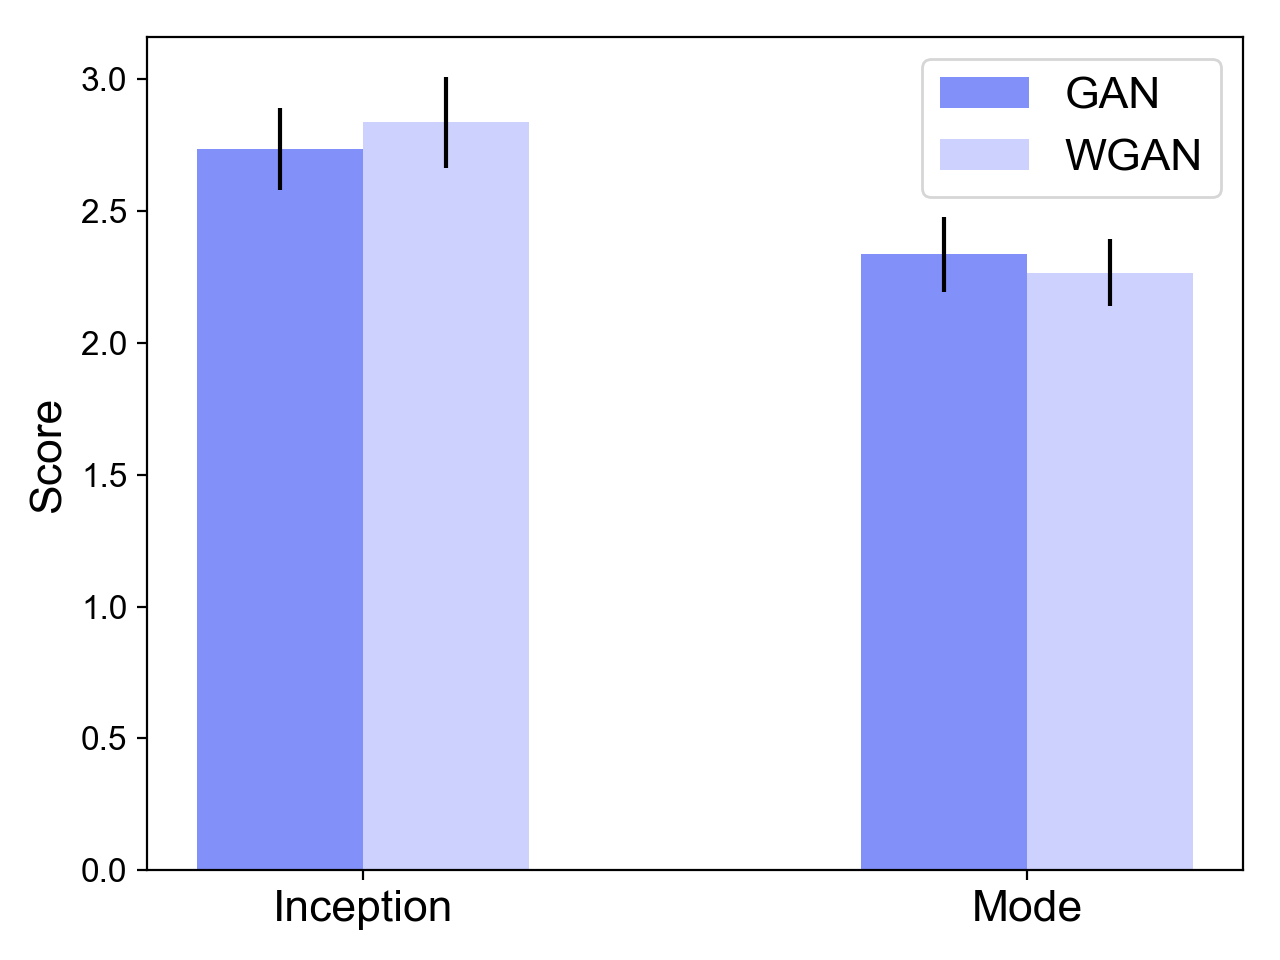
\includegraphics[scale=0.45]{imgs/score}
  \caption{Evaluating the performance of our trained GAN and WGAN using different metrics.}
\end{figure}

\subsection{Discussion on Scoring Methods}

The Inception score is
\begin{align*}
  \IS(P_g) = \exp\PARENS{\ex_{x\sim P_g} \big[\KL\big(p_M(y|x)\|p_M(y)\big)\big]}
\end{align*}
and the Mode score is
\begin{align*}
  \MS(P_g) = \exp\PARENS{\ex_{x\sim P_g} [\KL\big(p_M(y|x)\|p_M(y)\big)] - \KL\big(p_M(y) \| p_M(y^*)\big)},
\end{align*}
where $p_M(y|x)$ denotes the label distribution of $x$ as predicted by $M$, $p_M(y)$ is the marginal over the probability measure $P_g$ and $p_M(y^*)$ is the marginal over the real data.

One problem with the Inception score is that it only takes into account the ``crispness'' of the generated images, and leaves out whether the generating distribution actually ressembles that from the real data that we are trying to model. The Mode score corrects for this by adding the second $\KL$ term. We pay a small price in the time it takes to calculate this score however.

Taking this into account, we observe that our vanilla GAN model generates better images than our WGAN model, as reflected by the Mode score. This indicates that it better models the true data distribution, as compared to our WGAN model which has a higher Inception score.  Nonetheless, we should remain skeptical of this conclusion since a human observer would always prefer the samples from the GAN model than from the WGAN model.

\newpage
\bibliography{refs}
\bibliographystyle{iclr2017_conference}

\newpage
\appendix
\section{Generated Examples}
\begin{figure}[ht]
  \centering
  \begin{subfigure}{\textwidth}
    \centering
    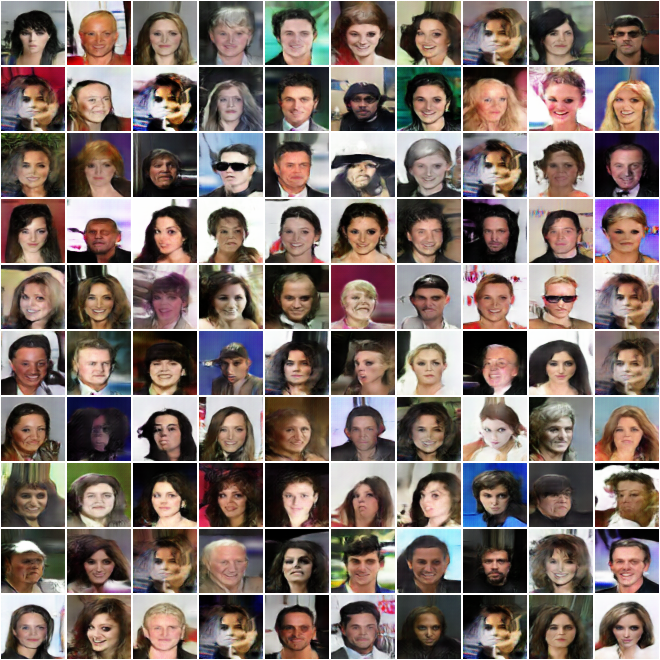
\includegraphics[scale=0.38]{imgs/gan_epoch50}
    \caption{Vanilla GAN}
  \end{subfigure}

  \vspace*{3mm}
  \begin{subfigure}{\textwidth}
    \centering
    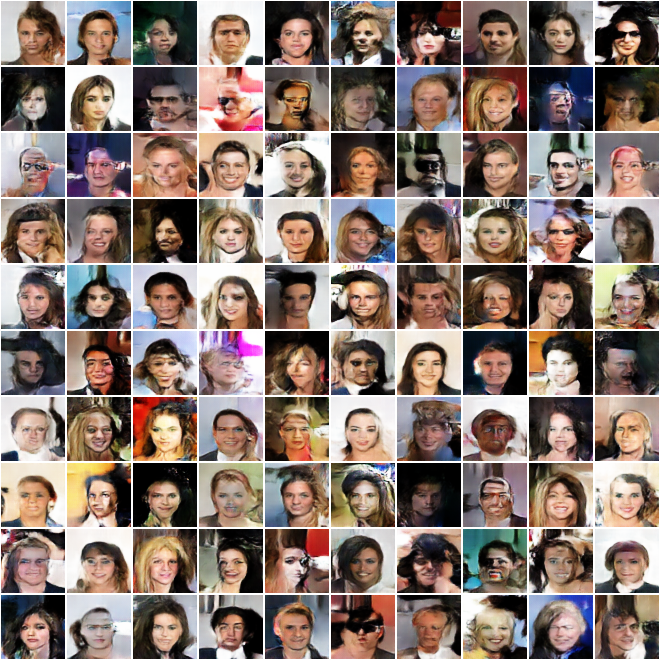
\includegraphics[scale=0.38]{imgs/wgan_epoch50}
    \caption{WGAN}
  \end{subfigure}
  \caption{100 generated images using both models trained for 50 epochs. All images look more or less plausible, but we can note a small mode collapse in the case of the vanilla GAN as multiple values of $\*z$ map to the same image (1,2). }
\end{figure}

\begin{figure}[ht]
  \centering
  \begin{subfigure}{\textwidth}
    \centering
    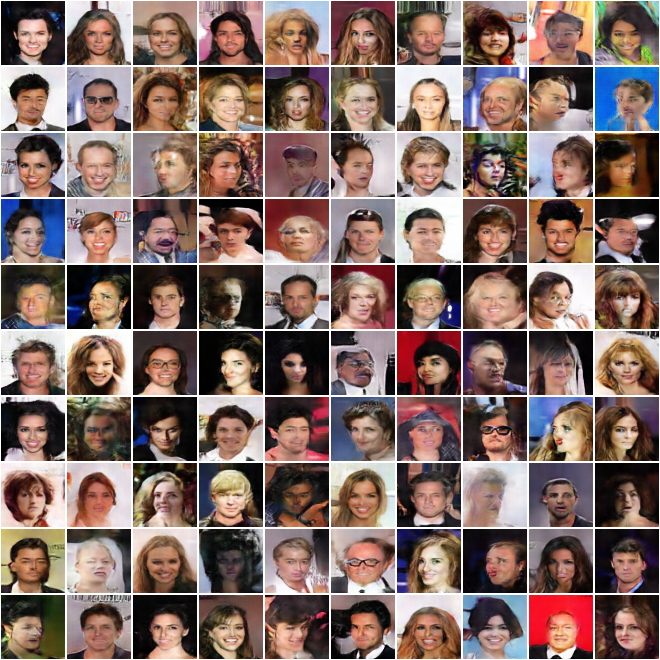
\includegraphics[scale=0.38]{imgs/lsgan_epoch44}
    \caption{LSGAN after 44 epochs}
  \end{subfigure}

  \vspace*{3mm}
  \begin{subfigure}{\textwidth}
    \centering
    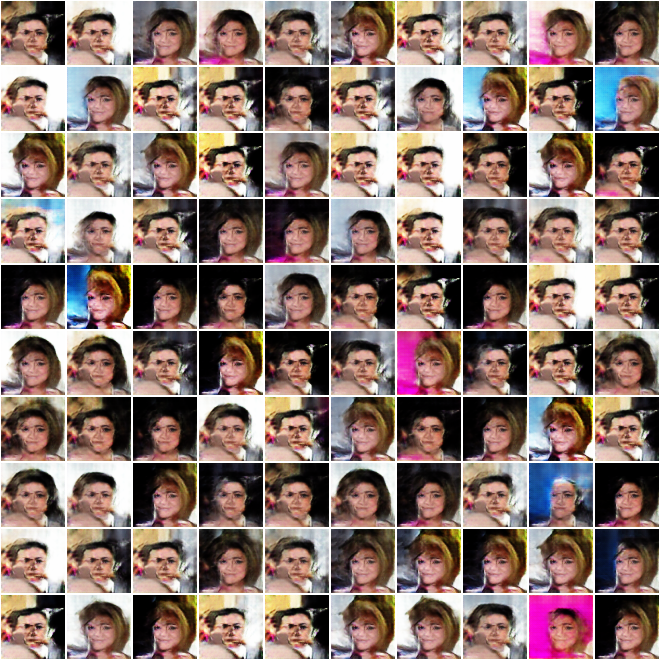
\includegraphics[scale=0.38]{imgs/lsgan_epoch50}
    \caption{LSGAN after 50 epochs}
  \end{subfigure}
  \caption{100 generated images using our trained LSGAN using the same hyperparameters as the vanilla GAN. Total mode collapse occurs at the end of training time.}
\end{figure}


\end{document}
